% Chapter Template

\chapter{Einleitung} % Main chapter title

\label{Chapter1} % Change X to a consecutive number; for referencing this chapter elsewhere, use \ref{ChapterX}

\lhead{Chapter 1. \emph{Introduction}} % Change X to a consecutive number; this is for the header on each page - perhaps a shortened title

%----------------------------------------------------------------------------------------
%	SECTION 1
%----------------------------------------------------------------------------------------
1. Satz:\\


\section{Motivation}
TODO: Motivation, Beispiel, Konventionen in Arbeit, Gliederung der Arbeit\\
Wo werden alles EventLogs benutzt? Erklären, warum es wichtig wäre, genau dort Constraints zu benutzen? Außer dem Verhindern von Betrug ist auch das Vermeiden von Fehlern wichtig. -\\
Um internen Betrug in Unternehmen zu verhindern, wird bei vielen Authorisierungsmodellen das separation of duty Prinzip beachtet. Dieses besagt, dass es bestimmte Aufgaben gibt, die nicht von ein un der selben Person erledigt werden können. Dazu gibt es verschiedene Ansätze, die ermögliche, Einschränkungen auf die Authorisierung zu definieren, die je nach Art bereits in der Entwurfphase des Workflows oder dynamisch während der Laufzeit erzwungen wird, indem sich die Informationen dynamisch aktualisieren (Hier ein paas Quellen angeben). Allerdings erlauben die aktuellen Modelle nur Einschränkungen innerhalb eines Workflows, was aber nicht ausreicheng ist.\\
Betrachten wir folgendes Beispiel:\\

\begin{figure}[ht]
	\centering
  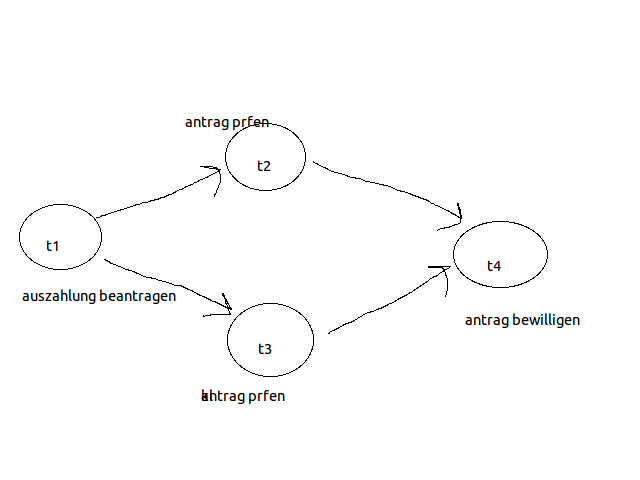
\includegraphics[width=0.9\textwidth]{Figures/Workflow}
	\caption{Workflow}
	\label{fig:Workflow}
\end{figure}

Um eine Zahlung zu tätigen, muss die Zahlung zuerst beantragt werden. Dieser Antrag muss zweimal geprüft werden. Sollte die Prüfung positiv verlaufen, wird der Antrag bewilligt und die Zahlung wird getätigt.

Es ist allerdings unerwünscht, dass t3 und t4 von der selben Person ausgeführt wird, die die Zahlung beantragt. Ferner sollten auch keine Verwandten dieser Person daran arbeiten, da die Bewilligung aus reiner Gefälligkeit erfolgen könnte.

Diese Einschränkungen, die sich jeweils auf einen Arbeitsablauf beziehen, sind aber nicht ausreichend, um Betrug zu verhindern. 
Es könnte sich eine Gruppe bilden, die sich in mehreren Instanzen des Arbeitsablaufs gegenseitig die Auszahlungen bewilligen.
Eine zusätzliche Einschränkung wäre somit, dass eine Gruppe nur 5mal an t1 und t2 zusammen arbeiten darf.





%-----------------------------------
%	Ziel der Arbeit
%-----------------------------------

\section{Ziel der Arbeit}

In dieser Arbeit wird eine Grammatik entwickelt, die es erlaubt, solche Einschränkungen zu definieren. Zusätzlich wird ein Programm vorgestellt, das MXML Logs einliest und sie auf die definierten Einschränkungen hin überprüft.



%-----------------------------------
%	AUFBAU DER ARBEIT
%-----------------------------------

\section{Aufbau der Arbeit}
Folgende Konventionen werden hier eingehalten: kursive Begriffe  bezeichnen Fachbegriffe, Blockschrift kennzeichnet Pseudocode,...
Begriffe, die zum ersten mal definiert werden, werden beim ersten Vorkommen \textbf{fett} geschrieben.

In Kapitel 2 werden wichtige Begriffe erläutert. In Kapitel 3 widmen wir uns der  Herleitung von Einschränkungen und der Definition einer antsprechenden Grammatik. Diese wird in Kapitel 4 in ein Programm integriert, welches Event Logs auf die Verletzung von Einschränkungen prüft. Dazu wird der Algorithmus vorgestellt. Kapitel 5 und 6 schließen mit einer Untersuchung der Korrektheit und einem Ausblick in weitere Forschung.

